\documentclass[../Final.tex]{subfiles}
\begin{document}
In this section, calculation results by numerical simulation would be presented. Discussion was presented based on each of applied configurations. 
Several responses on the struck ship was described and evaluated regarding influence degree of proposed parameters to the results. 

\subsection{Double hull size}

\begin{figure}[ht]
    \centering
    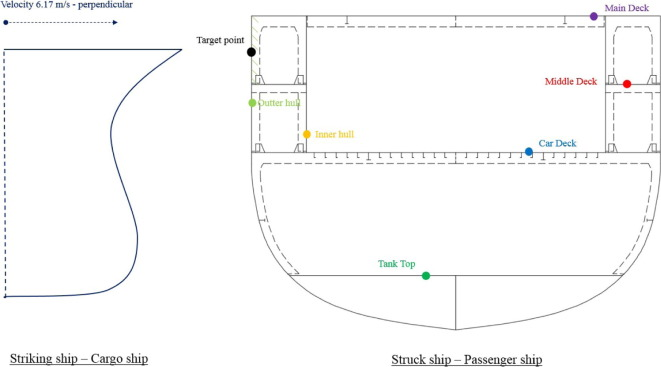
\includegraphics[width=\columnwidth]{fig4.jpg}
    \label{fig4}
    \caption{Illustration of side collision. Bullets highlight location of pointed components.}
\end{figure}

\begin{figure}[ht]
    \centering
    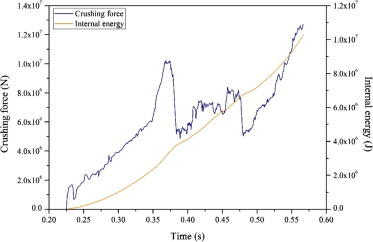
\includegraphics[width=\columnwidth]{fig5.jpg}
    \label{fig5}
    \caption{Crushing force and internal energy for double hull configuration 1.50m.}
\end{figure}

\begin{figure}[ht]
    \centering
    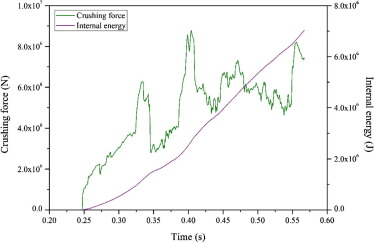
\includegraphics[width=\columnwidth]{fig6.jpg}
    \label{fig6}
    \caption{Crushing force and internal energy for double hull configuration 3.50m.}
\end{figure}

Safety standard of a ship against various forms of impact load (e.g. collision and grounding) can be evaluated from condition of the inner hull after resisting such damage. 
Breach of the inner hull can be considered fatal since damage occurs not only on ship structure, but also already reach ship cargo. Calculation results based on different hull configurations are presented in \ref{fig5} and \ref{fig6}. 
Internal energy in these graphs are defined as energy that is needed to plastically deform or even destroy the involved structures in impact. 
In this case, the struck ship as the deformable object is observed. Energy to deform side hull with narrower space was indicated higher as both hulls (outer and inner) were significantly damaged by the striking ship during penetration. 
Indication of higher internal energy is not solely dictated a structural configuration has better resistance against impact load. 
Crushing force in the figures is defined as force fluctuation during destruction of the involved objects take place by certain impact load. 
The force for wider space on the struck ship was observed go down in the end of collision process as the destruction was focussed on the outer hull. Major deformation or even hole on the inner hull could be 
avoided as large space was provided by double hull with size

\begin{figure}[ht]
    \centering
    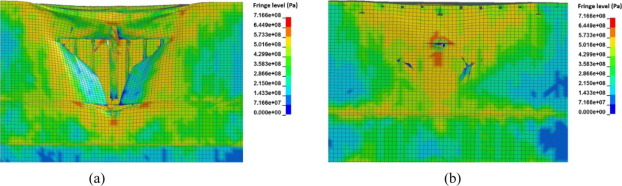
\includegraphics[width=\columnwidth]{fig7.jpg}
    \label{fig7}
    \caption{Damage pattern on the double hull structure with space 1.50 m: (a) outer hull, and (b) inner hull.}
\end{figure}

\begin{figure}[ht]
    \centering
    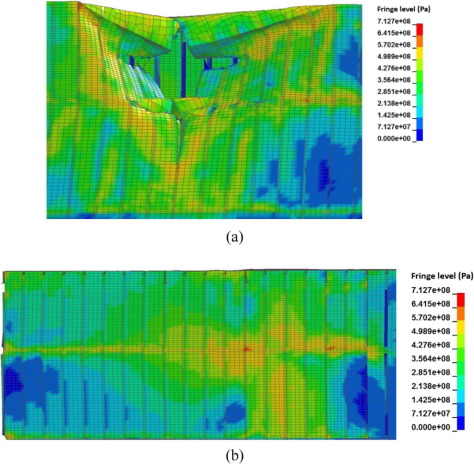
\includegraphics[width=\columnwidth]{fig8.jpg}
    \label{fig8}
    \caption{Damage pattern on the double hull structure with space 3.50 m: (a) outer hull, and (b) inner hull.}
\end{figure}

3.5 m in width. Contrast with this situation, the narrower dou-ble hull (1.5 m in width) showed rising trend line as penetration went further. 
This situation addressed the situation of the inner hull of this hull was slowly deformed plastically. Illustration of this phenomenon is presented in \ref{fig7} and \ref{fig8} for both hulls. 
The presented contours in these figures are von Mises stress which represent failure stress. In 1.5 m double hull, stress on the inner hull was found distributed on the area of penetrated hulls. 
Stress concentration was clearly indicating failure if pen­etration was continued on this location. 
Stress on inner was widely distributed on the inner hull for the larger double hull. This hull size provided adequate time during penetration to deliver the stress to other structural components. 
Initial conclusion based on this discussion that narrower double hull space more susceptible to failure during collision. 
Therefore, double hull with space 1.5 m would be used in further analyses and simulations accounting for material configurations. 

\subsection{Strength characteristic}

Material is inseparable element in structural analysis. In this work, this parameter is taken into consideration with deploying material with different strength magnitude. 
The energy results of this study indicated that the internal energy was equally perpendicular with magnitude of yield and ultimate strength. 
Material with higher strength needed more energy to be destroyed during penetration. Difference in yield strength between the first and second materials was found 12\% and internal energy introduced 12\% distinction. 
The third and fourth material showed difference 50 MPa in term of yield strength with energy comparison between both materials indicated 27\% discrepancy. Between the first and second materials, 

\begin{figure}[ht]
    \centering
    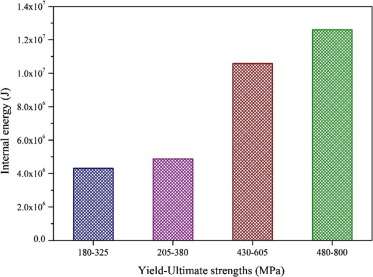
\includegraphics[width=\columnwidth]{fig9.jpg}
    \label{fig9}
    \caption{Internal energy for different applied material strength on the double hull structure.}
\end{figure}

\begin{figure}[ht]
    \centering
    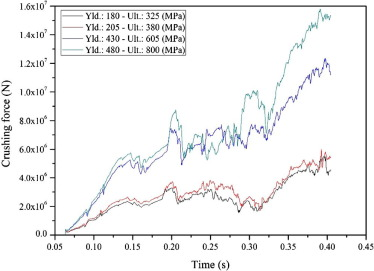
\includegraphics[width=\columnwidth]{fig10.jpg}
    \label{fig10}
    \caption{Characteristic of crushing force on the double hull structure with different strengths.}
\end{figure}

\begin{figure}[ht]
    \centering
    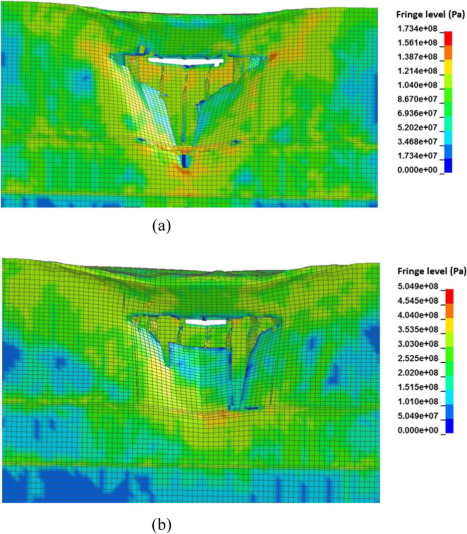
\includegraphics[width=\columnwidth]{fig11.jpg}
    \label{fig11}
    \caption{ Damage pattern on the outer and inner hulls: (a) yield 180 MPa, and (b) yield 480 MPa.}
\end{figure}

    
\begin{figure}[ht]
    \centering
    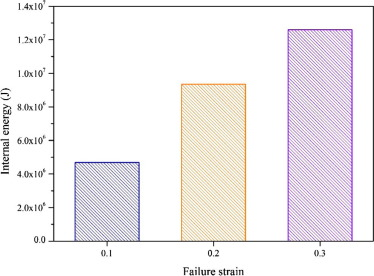
\includegraphics[width=\columnwidth]{fig12.jpg}
    \label{fig12}
    \caption{Effect of failure strain constant to internal energy during ship collision.}
\end{figure}

Difference was relative lower than the third and fourth materials, that contribution of tensile strength was taken into consideration as the third and fourth materials had bigger disparity. 
Behaviour of crushing force also provided good correlation since higher material strength, higher stress that would be experienced. These results are presented in \ref{fig9} and \ref{fig10}, consecutively. 
Damage extents in \ref{fig11} were presented by Tresca stress indicated that the higher strength would reduce casualties on the inner hull after collision process. 
This material was proven provide better resistance for side hull against collision by the striking ship. However, attention should be paid in term of material treatment. 
Higher strength tends to need more costly treatment in building and repairing processes which lead to increase of maintenance cost. 

\subsection{Failure strain}

In analysis using strain-dependent material to predict failure pattern on the involved objects, it was considered important to evaluate how far failure strain affected calculation results. 
Three different strain constants were applied on the deformable structure. 
Calculation results in \ref{fig12} indicated that the internal energy was gradually increasing for the proposed strain constants. 
The target structure was shown better strain capability during penetration and made the structure was harder to experience failure. Illustration in \ref{fig13} was presented wide area with was wrinkled as effect 
of collision load in structure with strain constant 0.3. Compared with the smallest constant which the inner hull was successfully breached and tearing was found that the striking ship cleanly tore the both hulls, 
the strain constant 0.3 delivered better capability to resist penetration by the striking ship. 
Benchmarking study can be considered as good method to estimate reasonable strain constant for applied material properties in analysis. 

\begin{figure}[ht]
    \centering
    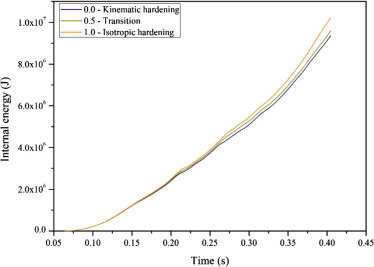
\includegraphics[width=\columnwidth]{fig14.jpg}
    \label{fig14}
    \caption{Internal energy for proposed assumption of yield surface. Significance is not found on the results.}
\end{figure}

\begin{figure}[ht]
    \centering
    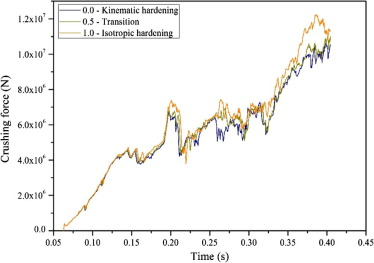
\includegraphics[width=\columnwidth]{fig15.jpg}
    \label{fig15}
    \caption{Crushing force during penetration by the striking ship with different assumed yield surfaces.}
\end{figure}

\subsection{Hardening value}

Hardening was taken into consideration to observe different assumption in position of yield surface during penetration. 
Kinematic hardening with constant 0 indicates that the radius of the yield surface is fixed but the center translates in the direction of the plastic strain, which means it can be move as translated direction of plastic strain. 
In opposite of the first assumption, if the yield surface is fixed and works as function of the plastic strain, this definition is called isotropic hardening with constant 1. 
The transition constant 0.5 was considered in the analysis to provide intermediary comparison for kinematic and isotropic results. 
In term of internal energy (\ref{fig14}), significant difference was unlikely found for all proposed assumptions. Trend line and value were also showing similarity in term of crushing force as presented in \ref{fig15}. 
Both responses indicated that isotropic hardening produced higher results than kinematic hardening with no remarkable characteristic. Results of the transition value 0.5 was found between kinematic and isotropic magnitudes. 

\end{document}